\documentclass[xcolor={dvipsnames,usenames}]{beamer}
%\documentclass[xcolor={dvipsnames,usenames},handout]{beamer} % use this to compile w/o pauses
\mode<presentation>
{
\usetheme{Madrid}
\usecolortheme{default}
\setbeamertemplate{itemize items}[default]
\setbeamertemplate{enumerate items}[default]
\setbeamercovered{transparent}
\usefonttheme[onlymath]{serif}
}


\usepackage{microtype}
\usepackage[normalem]{ulem}
%\usepackage{hyperref}
%\hypersetup{colorlinks=true, urlcolor=Blue, citecolor=Green, linkcolor=BrickRed, breaklinks, unicode}

\usepackage[nocompress]{cite}
\usepackage{amsmath,mathtools}
\usepackage{euscript}
\usepackage{latexsym}
\usepackage{amssymb,stmaryrd}
\usepackage{enumerate}
\usepackage{algorithm,algorithmicx}
\usepackage[noend]{algpseudocode}
\renewcommand{\algorithmicrequire}{\textbf{Requirement:}}

\usepackage{graphicx}
\usepackage{epstopdf}
\usepackage{subcaption}
\graphicspath{{./fig/}}


\title{Efficient Algorithms for Geometric Partial Matching}
\author[Allen Xiao]
{
	Pankaj~K.~Agarwal \and
	Hsien-Chih~Chang \and
	Allen~Xiao
}
\institute[SoCG 2019]
{
	Department of Computer Science, Duke University
}
\date{June 2019}

% tweak wd=X\paperwidth to modify the footer dimensions in the madrid theme
\makeatletter
\setbeamertemplate{footline}{
  \leavevmode%
  \hbox{%
  \begin{beamercolorbox}[wd=.25\paperwidth,ht=2.25ex,dp=1ex,center]{author in head/foot}%
    \usebeamerfont{author in head/foot}\insertshortauthor\expandafter\ifblank\expandafter{\beamer@shortinstitute}{}{~~(\insertshortinstitute)}
  \end{beamercolorbox}%
  \begin{beamercolorbox}[wd=.55\paperwidth,ht=2.25ex,dp=1ex,center]{title in head/foot}%
    \usebeamerfont{title in head/foot}\insertshorttitle
  \end{beamercolorbox}%
  \begin{beamercolorbox}[wd=.2\paperwidth,ht=2.25ex,dp=1ex,right]{date in head/foot}%
    \usebeamerfont{date in head/foot}\insertshortdate{}\hspace*{2em}
    \insertframenumber/\inserttotalframenumber \hspace*{2ex}
  \end{beamercolorbox}}%
  \vskip0pt%
}
\makeatother


% make tables less packed
\renewcommand{\arraystretch}{1.5}
% get rid of caption labels
%\setbeamertemplate{caption}{\raggedright\insertcaption\par}
%\captionsetup[subfigure]{labelformat=empty}
% set beamer highlight color (alert)
\setbeamercolor{alerted text}{fg=BrickRed}

\newcommand{\mycite}[1]{{\color{LimeGreen}\lbrack #1\rbrack}}
\newcommand{\etal}{\textit{et~al.}}
\newcommand{\softO}{\widetilde{O}}
\newcommand{\reals}{\mathbb{R}}
\newcommand{\ints}{\mathbb{N}}
\newcommand\nats{\mathbb{N}}
\newcommand{\eps}{\varepsilon}
\DeclareMathOperator{\polylog}{polylog}
\DeclareMathOperator{\poly}{poly}
\newcommand{\flr}[1]{{\lfloor #1\rfloor}}
\DeclareMathOperator*{\argmax}{arg\,max}
\DeclareMathOperator*{\argmin}{arg\,min}
\DeclareMathOperator{\Vor}{Vor}
\DeclareMathOperator{\VorRegion}{VorRegion}

\def\abs#1{\mathopen| #1 \mathclose|}		% use instead of $|x|$
\def\norm#1{\mathopen\| #1 \mathclose\|}	% use instead of $\|x\|$

\DeclareMathOperator{\cost}{cost}
\newcommand{\tsupply}{\lambda}
\newcommand{\fsupply}{\phi}

\newcommand{\A}{{\color{red}A}}
\newcommand{\B}{{\color{blue}B}}
\newcommand{\M}{\EuScript{M}}
\newcommand{\tildeM}{\widetilde{\EuScript{M}}}
\newcommand{\X}{\EuScript{X}}

\def\EMPH#1{\textcolor{BrickRed}{{\emph{#1}}}}



\begin{document}


\begin{frame}
\maketitle
\end{frame}

% INTRO

% 01: gentle example, emphasize cost fn
\begin{frame}{Geometric (bipartite) matching}
% two point sets in 2d, show cost fn (distance exponentitated to constant)
\begin{figure}
\begin{center}
\includegraphics<1>[width=0.8\textwidth,page=1]{example}%
\includegraphics<2>[width=0.8\textwidth,page=2]{example}%
\includegraphics<3->[width=0.8\textwidth,page=3]{example}%
\end{center}
\end{figure}

\end{frame}

\begin{frame}{Geometric (bipartite) partial matching}
% only k pairs
\begin{figure}
\begin{center}
\includegraphics<1->[width=0.8\textwidth,page=4]{example}%
\end{center}
\end{figure}
\end{frame}

% 03*: select prior work
\begin{frame}{Issues for geometric perfect matching algorithms}
% many other geometric matching algs need triangle ineq and fail for q > 1, e.g. certain embedding into sparse graph
% for some others, unclear how to generalize to partial (e.g. divide and conquer AV04)
% notable: SA12 (only first power)
\begin{equation*}
|A| = r, \quad |B| = n, \quad A, B \subset \reals^2, \quad q \geq 1
\end{equation*}
\begin{equation*}
\min_{k \text{-matching } M}\sum_{(a, b) \in M} \|a - b\|^q
\end{equation*}
\vspace{-10pt}
\begin{figure}
\begin{center}
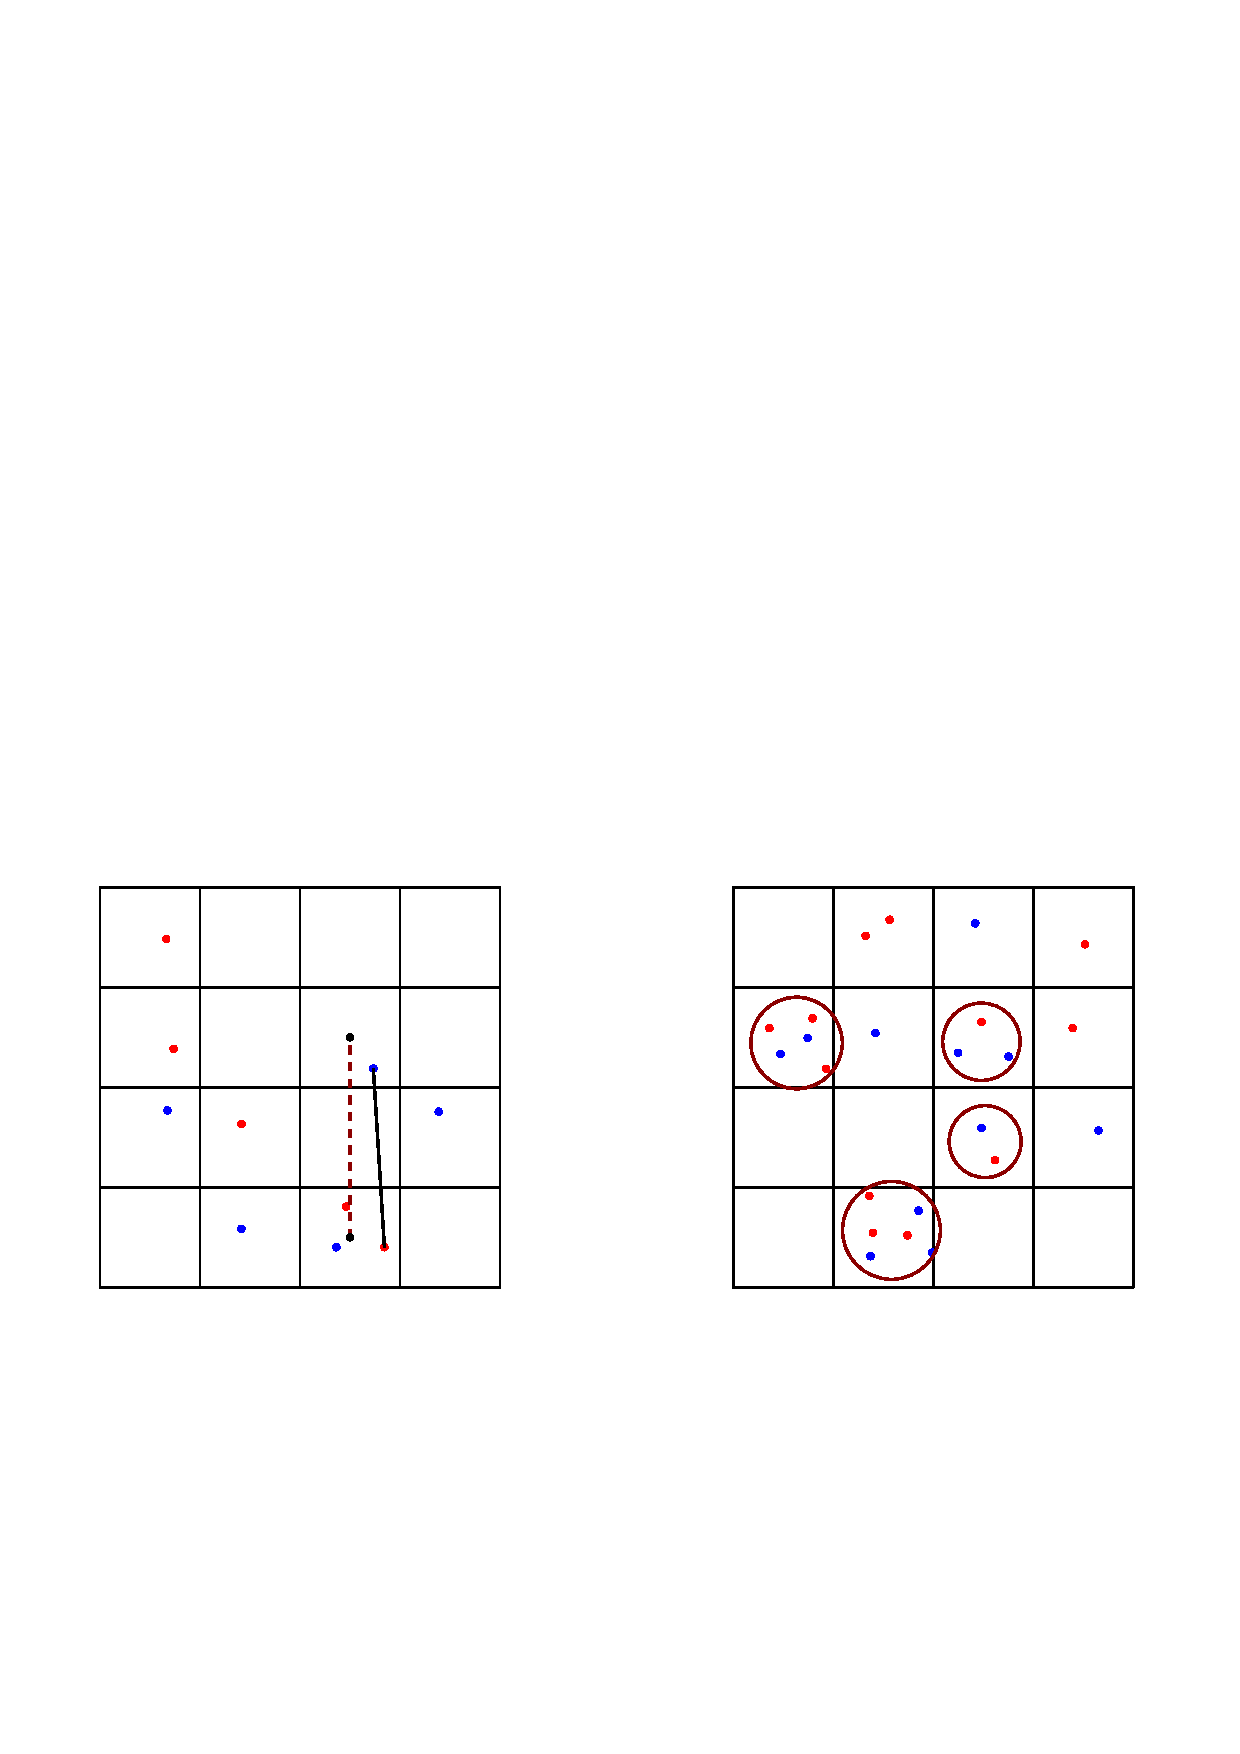
\includegraphics[width=0.9\textwidth,page=1]{perf_geom_issues}%
\end{center}
\end{figure}
\vspace{-5pt}
{\small For $q = 1$, [Sharathkumar-Agarwal]: $(1+\eps)$-approx. in $O(n\poly(1/\eps, \log n))$ time.}
\end{frame}

%TODO move this into a table
% 04: new results for partial, geom. based on prior work. present 1,2 only
\begin{frame}{Partial matching algorithms (non-geometric)}
% non-geom: Hungarian, RT/GHKT cost scaling,
% geometrized:
% Hungarian+BCP (Vaidya, KMRSS)
% cost-scaling+BCP
\begin{equation*}
|A| = r, \quad |B| = n, \quad A, B \subset \reals^2, \quad q \geq 1 
\end{equation*}
\begin{equation*}
\min_{k \text{-matching } M}\sum_{(a, b) \in M} \|a - b\|^q
\end{equation*}
\begin{itemize}
\item Hungarian algorithm [Kuhn]: $O(krn + k^2\log r)$
\item Cost-scaling [Ramshaw-Tarjan, Goldberg~\etal]: $O(rn\sqrt{k}\log(kC))$ (integer costs),
	or $O(rn\sqrt{k})$ time per cost scale.
\end{itemize}
\pause
\vspace{10pt}
Using dynamic bichromatic closest pair (BCP) data structures:
\begin{itemize}
\item Hungarian algorithm: $O(kn\polylog(n))$
\item Cost-scaling: $O(n\sqrt{k}\polylog(n))$ time per cost scale.
\end{itemize}
\end{frame}

% our results 1
\begin{frame}{Our results}
% Hungarian+BCP
% cost-scaling+BCP
Previous:
\begin{itemize}
\item Hungarian algorithm w/ BCP: $O(kn\polylog(n))$
\item Cost-scaling w/ BCP: $O(n\sqrt{k}\polylog(n))$ time per cost scale.
\end{itemize}
\pause
\vspace{10pt}

New:
\begin{enumerate}
\item Hungarian algorithm: $O((n+k^2)\polylog(n))$ time, exact.
\item Cost-scaling: $O((n+k\sqrt{k})\polylog(n))$ time per cost scale,
	$O(\log(n^q/\eps))$ scales, $(1+\eps)$-approx.
\pause
\vspace{10pt}
\item Geometric Transportation: $O(\min(n^2, nr^{3/2})\polylog(n))$ time, exact.
\end{enumerate}
\end{frame}

% HUNG

% 05: Hungarian algorithm and least-cost augmentation
\begin{frame}{Hungarian algorithm}
\vspace{-10pt}
\begin{figure}
\begin{center}
\includegraphics<1>[width=0.8\textwidth,page=1]{hung_example}%
\includegraphics<2>[width=0.8\textwidth,page=2]{hung_example}%
\includegraphics<3>[width=0.8\textwidth,page=3]{hung_example}%
\includegraphics<4>[width=0.8\textwidth,page=4]{hung_example}%
\includegraphics<5>[width=0.8\textwidth,page=5]{hung_example}%
\includegraphics<6>[width=0.8\textwidth,page=6]{hung_example}%
\includegraphics<7>[width=0.8\textwidth,page=7]{hung_example}%
\includegraphics<8->[width=0.8\textwidth,page=8]{hung_example}%
\end{center}
\end{figure}
\vspace{-15pt}
\onslide<9->{Hungarian algorithm:}
\begin{enumerate}
\item<9-> \alert{Hungarian search}: Dijkstra-like search changing $\pi$ until $\exists$ an admissible augmenting path.
\item<9-> Augment by the admissible augmenting path you found.
\end{enumerate}
\end{frame}

% 06: Hungarian search with BCP
\begin{frame}{Hungarian search}
\begin{itemize}
\item \alert{Reduced cost}: $c_\pi(v, w) = c(v, w) - \pi(v) + \pi(w)$
\item Keep $\pi$ feasible --- $c_\pi(v, w) \geq 0$ for all residual arcs $(v, w)$.
\item \alert{Admissible}: $c_\pi(v, w) \leq 0$ for residual arc $(v, w)$.
\end{itemize}
\begin{figure}
\begin{center}
\includegraphics<1>[width=0.8\textwidth,page=9]{hung_example}%
\includegraphics<2>[width=0.8\textwidth,page=10]{hung_example}%
\includegraphics<3>[width=0.8\textwidth,page=11]{hung_example}%
\includegraphics<4>[width=0.8\textwidth,page=12]{hung_example}%
\includegraphics<5>[width=0.8\textwidth,page=13]{hung_example}%
\includegraphics<6>[width=0.8\textwidth,page=14]{hung_example}%
\includegraphics<7>[width=0.8\textwidth,page=15]{hung_example}%
\includegraphics<8>[width=0.8\textwidth,page=16]{hung_example}%
\includegraphics<9>[width=0.8\textwidth,page=17]{hung_example}%
\includegraphics<10->[width=0.8\textwidth,page=18]{hung_example}%
\end{center}
\end{figure}
\end{frame}

\begin{frame}{Hungarian search, with BCP}
\begin{itemize}
\item<1-> ``What is the minimum reduced cost residual arc leaving $X$?''
\item<1-> For $B \to A$ residual arcs, min-heap over matching edges (at most $k$).
\item<1-> For $A \to B$ residual arcs\ldots \onslide<2->{\alert{bichromatic closest pair} between $A \cap X$ and $B \setminus X$.}
\begin{figure}
\begin{center}
\includegraphics<1>[width=0.8\textwidth,page=1]{bcp}%
\includegraphics<3->[width=0.8\textwidth,page=2]{bcp}%
\end{center}
\end{figure}
\item<4-> {[Kaplan~\etal~17]}: For points in $\reals^2$, insert/delete in $O(\polylog n)$ time, query BCP in $O(\log^2 n)$ time.
\end{itemize}

\end{frame}

% 08*: problem: initializing the BCP data structure (why not persistence?)
\begin{frame}{Problem: BCP initialization}
\begin{itemize}
\item $k$ augmentations
\item Goal: $O(k\polylog n)$ time per augmentation
\pause
\item $O(k)$ relaxations per Hungarian search (at most $k$ matching edges)
\pause
\item But, the initial BCP data structure of each Hungarian search has size $O(n)$.
\pause
\item \ldots $O(kn\polylog n)$ time so far.
\end{itemize}
\end{frame}

% 09*: rewinding --> k^2polylogn time per augmentation, one-time npolylogn pre
\begin{frame}{Rewinding}
\begin{itemize}
\item Initial $X$ is the set of unmatched $A$ vertices.
\pause
\item Initial $X$ loses exactly one vertex after an augmentation.
\end{itemize}
\pause
\vspace{10pt}
\begin{enumerate}
\item Record the BCP operations we did during the Hungarian search, then
	\alert{rewind} them to recover the initial BCP state.
\pause
\item Delete one more point from the BCP to get the next initial state.
\end{enumerate}
\pause
\vspace{10pt}
\begin{itemize}
\item $O(k\polylog n)$ time to rewind.
\pause
\item Build the whole BCP once ($O(n\polylog n)$), reuse every augmentation.
\pause
\item Persistence?\\
\pause
Unfortunately, the BCP insert/delete bounds are amortized.
\end{itemize}
\end{frame}

% 10: potential changes + Vaidya?
\begin{frame}{Efficient potential updates}
\begin{itemize}
\item During the Hungarian search, how do we have time to raise $\pi$ for every $v \in X$?
\pause
\item {[Vaidya 89]}: batch changes into a single variable $\delta$.\\
	``Raise $\pi$ for every $v \in X$ by $\alpha$'' replaced by $\delta \gets \delta + \alpha$.
\vspace{10pt}
\pause
\item When a point enters $X$ we save it with $\gamma(v) \gets \pi(v) - \delta$.
\pause
\item At any point, $\pi(v) = \gamma(v) + \delta$ for $v \in X$.
\vspace{10pt}
\pause
\item To use with rewinding, don't reset $\delta$ between augmentations.
\vspace{10pt}
\pause
\item Summary: Build the BCP once ($O(n\polylog n)$).
	Each Hungarian search and augmentation takes $O(k\polylog n)$ time.
	$O((n+k^2)\polylog n)$ time total.
\end{itemize}

\end{frame}

% COST-SCALE

% our results 2
\begin{frame}{Our results}
% Hungarian+BCP
% cost-scaling+BCP
New:
\begin{enumerate}
\item<0> Hungarian algorithm: $O((n+k^2)\polylog(n))$ time, exact.
\item<1-> Cost-scaling: $O((n+k\sqrt{k})\polylog(n))$ time per cost scale,
	$O(\log(n^q/\eps))$ scales, $(1+\eps)$-approx.
\vspace{10pt}
\item<0> Geometric Transportation: $O(\min(n^2, nr^{3/2})\polylog(n))$ time, exact.
\end{enumerate}
\end{frame}

% 02: unit-cap MCF form
\begin{frame}{Geometric partial matching as unit-capacity min-cost flow}
% unit-capacity construction, note number of edges
\begin{figure}
\begin{center}
\includegraphics<1>[width=\textwidth,page=1]{pm-to-mcf}%
\includegraphics<2>[width=\textwidth,page=2]{pm-to-mcf}%
\includegraphics<3>[width=\textwidth,page=3]{pm-to-mcf}%
\includegraphics<4>[width=\textwidth,page=4]{pm-to-mcf}%
\includegraphics<5>[width=\textwidth,page=5]{pm-to-mcf}%
\includegraphics<6>[width=\textwidth,page=6]{pm-to-mcf}%
\includegraphics<7>[width=\textwidth,page=7]{pm-to-mcf}%
\includegraphics<8->[width=\textwidth,page=8]{pm-to-mcf}%
\end{center}
\end{figure}
\end{frame}

% 11: cost-scaling unit-cap MCF
\begin{frame}{Partial matching by cost-scaling}
\begin{itemize}
\item Reduced cost: $c_\pi(v, w) = c(v, w) - \pi(v) + \pi(w)$
\item<0> Keep $\pi$ feasible --- $c_\pi(v, w) \geq 0$ for all residual arcs $(v, w)$.
\item \alert{$\theta$-optimal}: $c_\pi(v, w) \geq -\theta$ for all residual arcs $(v, w)$.
\item Admissible: $c_\pi(v, w) \leq 0$ for residual arc $(v, w)$.
\end{itemize}
\pause
\begin{lemma}
A $\theta$-optimal circulation for the partial matching network has cost at most $c(f^*) + 6k\theta$.
\end{lemma}
\pause
\begin{itemize}
\item Find $\theta$-optimal circulations for shrinking values of \alert{scale} $\theta$.
\end{itemize}
\end{frame}

\begin{frame}{Partial matching by cost-scaling}
Given a $2\theta$-optimal circulation from the previous scale,
\pause
\begin{enumerate}
\item Find a $\theta$-optimal pseudoflow $f$ with $O(k)$ excess.
\pause
\item \alert{Refine} $f$ into a $\theta$-optimal circulation.
\end{enumerate}
\pause
\begin{lemma}
Can reduce $(1+\eps)$-approx. geometric partial matching to executing
$O(\log(n^q/\eps))$ scales of the cost-scaling algorithm.
\end{lemma}
\pause
\begin{itemize}
\item Focus on solving each scale efficiently.
\end{itemize}
\end{frame}

% 12: changing scales (2\eps to \eps, losing circulation)
\begin{frame}{Initial $\theta$-optimal pseudoflow of a scale}
\begin{figure}
\begin{center}
\includegraphics<1>[width=0.8\textwidth,page=1]{scale_init}%
\includegraphics<2>[width=0.8\textwidth,page=2]{scale_init}%
\includegraphics<3->[width=0.8\textwidth,page=3]{scale_init}%
\end{center}
\end{figure}
\begin{itemize}
\item<1-> Input circulation: $c_\pi(v, w) \geq -2\theta$ for all residual arcs.
\item<2-> Forward arcs have reduced cost raised by $+\theta$ --- must be $\theta$-optimal.
\item<3-> Only $O(k)$ reverse arcs, so check each one manually.
\end{itemize}
\end{frame}

% 13: refinement by blocking flows (more of the same, \sqrt{k} per scale, O(k) size per blocking)
\begin{frame}{Refinement by blocking flows}
\begin{enumerate}
\item \alert{Hungarian search}:
	\onslide<0>{Dijkstra-like search changing $\pi$ until $\exists$ an admissible augmenting path.}\\
	Dijkstra-like search changing $\pi$ \alert{in units of $\theta$} until $\exists$ an admissible augmenting path.
\item \onslide<0>{Augment by the admissible augmenting path you found.}\\
	Augment by an admissible \alert{blocking flow} $g$.\\
\begin{figure}
\begin{center}
\includegraphics<1>[width=0.8\textwidth,page=1]{blocking_flow}%
\includegraphics<2>[width=0.8\textwidth,page=2]{blocking_flow}%
\includegraphics<3>[width=0.8\textwidth,page=3]{blocking_flow}%
\includegraphics<4->[width=0.8\textwidth,page=4]{blocking_flow}%
\end{center}
\end{figure}
	\begin{itemize}
	\item<5-> Find by DFS through the admissible residual arcs.
	\end{itemize}
\end{enumerate}
\end{frame}

\begin{frame}{Refinement by blocking flows}
\begin{enumerate}
\item \alert{Hungarian search}: Dijkstra-like search changing $\pi$
	\alert{in units of $\theta$} until $\exists$ an admissible augmenting path.

\item Augment by an admissible \alert{blocking flow} $g$.
\vspace{10pt}
\begin{lemma}
After $O(\sqrt{k})$ blocking flows, $f$ is a circulation.
\end{lemma}
\end{enumerate}
\end{frame}

% 14*: new problem: number of relaxations could be \Omega(n) (example); compare vs Hung
\begin{frame}{Hungarian search dead ends}
\begin{itemize}
\item There can be $\Omega(n)$ relaxations even if $k$ is very small.
\begin{figure}
\begin{center}
\includegraphics<1>[width=0.9\textwidth,page=1]{why_dead}%
\includegraphics<2>[width=0.9\textwidth,page=2]{why_dead}%
\includegraphics<3>[width=0.9\textwidth,page=3]{why_dead}%
\includegraphics<4->[width=0.9\textwidth,page=4]{why_dead}%
\end{center}
\end{figure}
\end{itemize}
\end{frame}

% 15: dead/alive nodes, alive paths. "really want to query minimizing alive path instead", "don't track their potential"
\begin{frame}{Dead or alive}
\begin{itemize}
\item \alert{Alive nodes}: nonzero excess/deficit, or adjoining flow support arcs.
\item \alert{Dead nodes}: ones which aren't alive.
\begin{figure}
\begin{center}
\includegraphics<1>[width=0.8\textwidth,page=5]{why_dead}%
\includegraphics<2>[width=0.8\textwidth,page=6]{why_dead}%
\includegraphics<3,4>[width=0.8\textwidth,page=7]{why_dead}%
\includegraphics<5>[width=0.8\textwidth,page=8]{why_dead}%
\includegraphics<6->[width=0.8\textwidth,page=9]{why_dead}%
\end{center}
\end{figure}
\item<4-> \alert{Alive path}: residual path between two alive nodes with no other alive nodes in between.
\item<7-> Don't need to track potential of dead nodes.
\end{itemize}
\end{frame}

% 16: alive paths in the BCP
\begin{frame}{Hungarian search over alive paths}
\begin{itemize}
\item Alive paths have length 1, 2, or 3.
\begin{figure}
\begin{center}
\includegraphics<1>[width=0.8\textwidth,page=1]{alive_paths}%
\includegraphics<2>[width=0.8\textwidth,page=2]{alive_paths}%
\includegraphics<3>[width=0.8\textwidth,page=3]{alive_paths}%
\includegraphics<4>[width=0.8\textwidth,page=4]{alive_paths}%
\includegraphics<5->[width=0.8\textwidth,page=5]{alive_paths}%
\end{center}
\end{figure}
\item<5-> Telescoping on alive paths: $c_\pi(s \to a \to b) = c(a, b) - \pi(s) + \pi(b)$
\item<6-> Can still use BCP.
\end{itemize}
\end{frame}

% 17: # relaxations = O(|supp(f)|) = O(k)
\begin{frame}{How many relaxations now?}
\begin{itemize}
\item $O(k)$ alive nodes.
\item Every alive path relaxation adds another alive node to $X$.
\item Thus, $O(k)$ relaxations.
\end{itemize}
\end{frame}

% 18*: dead node potentials
\begin{frame}{Dead node potentials}
\begin{itemize}
\item Dead nodes may become alive again after an augmentation.
\item Also, at the end of a scale, we need potentials for all nodes.
\item What's the right value for a dead node's potential?
\vspace{10pt}
\pause
\begin{equation*}
\pi(v) = \begin{cases}
	\pi(s) & v \in A\\
	\pi(t) & v \in B
\end{cases}
\end{equation*}
\pause
\item This choice preserves $\theta$-optimality and ensures that the component
	arcs of an admissible alive path are admissible.
\end{itemize}
\end{frame}

% 19: punchline running time: per-scale npolylogn pre, k\sqrt{k}polylogn per, O(log(n^q/\eps)) scales
\begin{frame}{Cost-scaling time summary}
\begin{itemize}
\item $O(\log(n^q/\eps))$ scales.
\item $O(\sqrt{k})$ iterations of refinement.
\item Each blocking flow has size $O(k)$.
\vspace{10pt}
\pause
\item Combine alive paths with previous ideas: rewinding and batched potential updates.
\pause
\item $O(k\polylog n)$ time for each Hungarian search and DFS (finding blocking flow).
\pause
\item $O(n\polylog n)$ to build the initial BCP data structures per scale.
\vspace{10pt}
\pause
\item $O((n+k\sqrt{k})\polylog n)$ time per scale, $O(\log(n^q/\eps))$ scales, $(1+\eps)$-approx.
\end{itemize}
\end{frame}

% end slide
\begin{frame}{The End}
\begin{center}
	Thank you.
\end{center}
\end{frame}



%SECTION: pmt

% gentle example + equation

%\begin{frame}{Example}
%\begin{figure}
%\begin{center}
%\includegraphics<1>[width=\textwidth,page=1]{pmt_example}%
%\includegraphics<2>[width=\textwidth,page=2]{pmt_example}%
%\includegraphics<3>[width=\textwidth,page=3]{pmt_example}%
%\includegraphics<4>[width=\textwidth,page=4]{pmt_example}%
%\includegraphics<5>[width=\textwidth,page=5]{pmt_example}%
%\includegraphics<6>[width=\textwidth,page=6]{pmt_example}%
%\includegraphics<7->[width=\textwidth,page=7]{pmt_example}%
%\end{center}
%\end{figure}
%\begin{itemize}
%\item<7-> Find the minimum-cost matching over all translations.
%\end{itemize}
%\end{frame}


%\begin{frame}[allowframebreaks]{Citations}
%\tiny
%\bibliography{ref}
%\bibliographystyle{alpha}
%\end{frame}

\end{document}
